\documentclass[conference]{IEEEtran}
\usepackage[english]{babel}
\usepackage{cite,setspace}
\usepackage[autostyle]{csquotes}
\usepackage{amsmath,amssymb,amsfonts}
\usepackage{algorithmic}
\usepackage{graphicx}
\graphicspath{{images/}}
\usepackage{textcomp}
\usepackage{xcolor}
\usepackage[outputdir=output]{minted}
%\usemintedstyle{autumn} % friendly, colorful
%\newminted{c}{mathescape, linenos, numbersep=5pt, gobble=0, frame=lines, framesep=2mm}
%\definecolor{background}{gray}{0.90}
%\newminted{bash}{bgcolor=background}
%\newminted{console}{bgcolor=background}
%\usemintedstyle[console]{bw}
\def\BibTeX{{\rm B\kern-.05em{\sc i\kern-.025em b}\kern-.08em
    T\kern-.1667em\lower.7ex\hbox{E}\kern-.125emX}}
\begin{document}

\title{Dynamic Frame Generation Using Machine Learning
and Scene Data
}

\author{\IEEEauthorblockN{Mark Wesley Harris}
Dr. Sudhanshu Semwal, CS 5790\\
University of Colorado\\
at Colorado Springs\\
May 16, 2019}

\maketitle

\begin{abstract}
This paper describes my preliminary research and implementation of a
system for dynamically generating frames or portions of frame
of a given animation.
\end{abstract}

\section{Introduction}
\label{sec:introduction}
Rendering the frames of a production-level quality animation can take an
excessive amount of time. As stated in \cite{ref:monsters}, ``All told, it has
taken more than 100 million CPU hours to render [Monster's University] in its final form. If
you used one CPU to do the job, it would have taken about 10,000 years to
finish. With [the supercomputer]\dots it took a couple of years to
render.'' The slowness of high quality rendering is all the more pertinent when considering all of the
pre-film preduction, such as intermediate renderings, changes to the scene, and
recasting or changes in the script. If there was a way to speed up the rendering
process, it would greatly benefit feature film animation and 3D effects companies such as Pixar
and Industrial Light \& Magic.

So how might we be able to speed up rendering? The main bottleneck that
researchers of this topic have been struggling with is the level of detail
encapsulated within a single frame of an animation. For example of this, Figure
\ref{fig:incredibles} shows a close up of of Bob Parr's shirt from the trailer
of ``Incredibles 2'' (released by Pixar June 15, 2018). There is enough
resolution on that image to clearly show not only the detailed stitching of the
fabric, but also strands of thread extruding from the shirt itself. While a
viewer most likely won't be able to discern these details during the running
movie, the quality tricks their subconscious into believing they are
experiencing something real; these details help convey more emotion and
connections to the world inhabited by the characters on the screen.

\begin{figure}[htbp]
\centerline{
\includegraphics[width=8cm]{incredibles.png}}
\caption{Level of detail in Pixar's ``Incredibles 2''.}
\label{fig:incredibles}
\end{figure}

\subsection{Problem Statement}
\label{subsec:problem_statement}
So if this bottleneck cannot be surpassed by lowering the quality, perhaps we
can overcome it through rendering less frames. This is the foundationary concept
of my project. The production pipeline would work as follows:

\begin{enumerate}
\item Artists create content as they would normally.
\item When the animation is ready to be rendered as a video, only every other
frame is rendered.
\item These frames, are then passed into a preprocessing stage to generate
what I call
``frameblocks'' (see Section \ref{subsec:frameblocks} for more information).
\item Scene data for each frameblock is extracted.
\item All collected frameblock/scene data pairs are passed into a generator/discriminator
Machine Learning architecture (see Figure \ref{fig:block_diagram}) to train an algorithm
to recognize the relationships between the rendered frame and scene data.
\item Once the algorithm is sufficiently trained, scene data for the missing
frames is input into the generator system in order to create frameblocks
representing the previously unseen rendered frame.
\item These generated frameblocks are stitched together (perhaps using another Machine
Learning model) in order to output a final rendered frame.
\end{enumerate}

There are many benefits to using this system. The most obvious is the ability
for artists to select the frames that are input into the algorithm; using half
of an animation's frames guarantees most changes will be captured in the
generated frameblocks, however artists may also include frames that have
uniqueness they would want to be recognized by the algorithm. Another benefit is
the ability to apply the trained model to similar 3D scenes, or to small changes
of the trained 3D scene. Thus the animation pipeline itself could be sped up
significantly by rendering predictions of how an animated scene will look in
realtime.

My hypothesis is that using the system outlined in this paper, rendering the
final animation will take less time than it does currently and animators will
have more flexibility for predicting what their animations will look like once
rendered. For this paper I first in Section \ref{sec:related_concepts} work
related to my project, then provide an overview
of my proposed architecture in \ref{sec:architecture}. Section
\ref{sec:considerations} presents what I focused on for this term, and finally
Section \ref{sec:implementation} I then discuss what I implemented.
I conclude with Section \ref{sec:future_work} to discuss my plans for the future of
the project.

\section{Related Concepts}
\label{sec:related_concepts}
I found found many research concepts, especially those relating to Machine Learning,
which provide the foundations for implementating this project.
In Section \ref{subsec:applicable} I discuss the
research (much of it cutting-edge) which has provided me insight into the
components that make up the final architecture I will implement and evalulate.
Then in Section \ref{subsec:complex_systems} I
touch on concepts from Complex Systems to discuss the relationships between
the 3D animated scene and dynamism, and the complexities of what needs to be
recognized by the Machine Learning models.

\subsection{Applicable research}
\label{subsec:applicable}
I have found many papers that are applicable to my stated problem. I would like
to discuss 4 of them in detail as well as provide
discussion on how they could be applied to my project implementation.

\cite{ref:frame_prediction} (``Geometry-Based Next Frame Prediction From
Monocular Video'') focuses on generating the
next frame of a monocular (i.e. single-view) video 
given the video's previous frames. The researchers deployed
an LSTM Machine Learning model in order to generate a depth map representing the next frame.
Another Machine Learning model was then applied to convert the generated depth
map into the pixels of the predicted frame. The largest deficiency of their
project was the poorness of the output frame's quality as shown in Figure
\ref{fig:frame_prediction}; in order to use their
application for production-quality outputs, more steps would have
to be taken to ensure the quality is comparable to the quality of the original input frames.
Concerning applications to my
project, what was most note-worthy is the use of the LSTM model in order to
collect changes from all previous frames instead of just one previous frame;
I feel this type of mechanism will be
crucial for the generative model described in Section \ref{sec:architecture}.

\begin{figure}[htbp]
\centerline{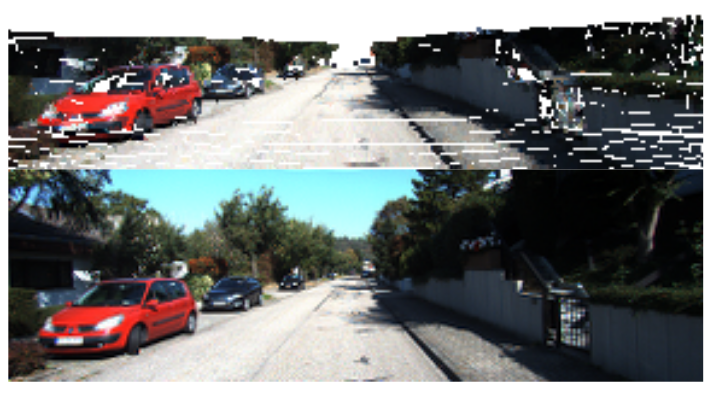
\includegraphics[width=8cm]{frame_prediction.png}}
\caption{Example of output frame and depth map of \cite{ref:frame_prediction}.}
\label{fig:frame_prediction}
\end{figure}

\cite{ref:spatiotemporal} (``Spatiotemporal Variance-Guided Filtering: Real-Time Reconstruction for
Path-Traced Global Illumination'') concentrates on
generating high quality outputs given very low quality input
frames. The inputs to the algorithm are rendered frames using one path-per-pixel global
illumination. As shown in Figure \ref{fig:spatiotemporal}, they are able to
transform very crude, noisy frames into production-grade outputs comparable to
the frames rendered at full resolution. Their algorithm is essentially a
multi-pass filter which the inputs are fed into, making it very fast and
reliable. My project benefit's from the foundational algorithms presented in
this research, however the overall premises are very different; my problem
requires frame generation given scene data that has not been rendered at all,
while theirs depends on entire rendered frames.

\begin{figure}[htbp]
\centerline{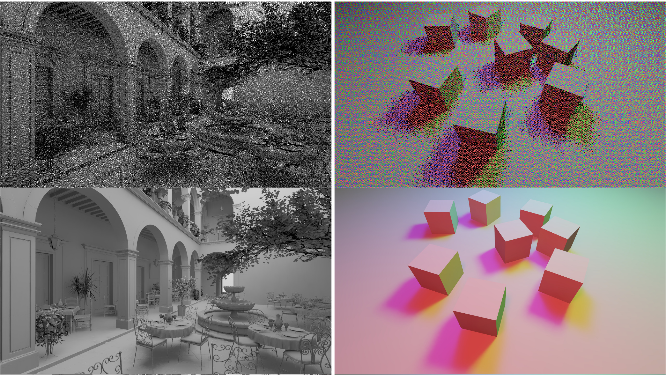
\includegraphics[width=8cm]{spatiotemporal.png}}
\caption{Example input and output frame of \cite{ref:spatiotemporal}.}
\label{fig:spatiotemporal}
\end{figure}

\cite{ref:posecnn} (``PoseCNN: A Convolutional Neural Network for 6D Object Pose Estimation in
Cluttered Scenes'', 2018) proposes a framework called ``PoseCNN'' which
employes a CNN to estimate pose information and object attributes given an input
image. The general architecture is shown in Figure \ref{fig:posecnn}; an image
is input into the system, and what is output are semantic labels, 3D
translation, and 3D rotation of each object. The researchers deem the collection
of these outputs ``6D'' data, since there are 6 dimensions total. This
research is very applicable to my project, since I need to generate some form of
the same information about objects in a 3D scene to use as inputs into my
system. I will consider the author's references and reasoning when making those
decision for the scene data inputs of my project.

\begin{figure}[htbp]
\centerline{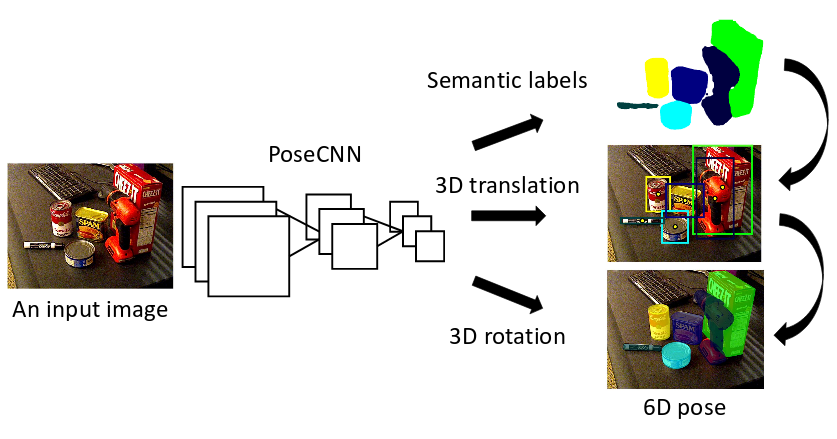
\includegraphics[width=8cm]{posecnn.png}}
\caption{Example architecture for \cite{ref:posecnn}.}
\label{fig:posecnn}
\end{figure}

\cite{ref:pose_guided} (``Pose Guided Person Image Generation'', 2017)
presents a system entitled
``Pose Guided Person Generation Network'' (abbreviated as
PG\textsuperscript{2}). This system takes as input a condition image
of a person in a given pose, and an image representing the targe pose the person
should be translated into (the choice of the representation for pose data is explained further in the
paper). Using two difference generators,
the system produces as intermediate output a low-resolution generated
image that defines global structure and features for the new pose, as well as a final refined
image of the person in the new pose (see Figure \ref{fig:pose_guided} for
details on their project architecture). I found this research directly applicable
to my project, since both problems involve combining an image with extraneous data. There are, however,
some differences between my project and theirs. As explained more in their
paper, the authors were able to represent pose data as a standardized black and white image.
Since my project requires the use of scene data outside of the rendered
boundaries (i.e. what the camera can ``see''), I would find it difficult to
obtain good results with the same approach. As I also found with the research in
\cite{ref:spatiotemporal}, this project requires an input image while the only
input of my final generative architecture is scene data itself. I will need to
keep this in mind during my investigation of what Machine Learning models to
develop for the generator. Despite these counterpoints, I do find the overall
system achitecture to most closely represent my target architecture; I plan to
have two generators and one discriminator, which can be trained on frame and
scene inputs.

\begin{figure}[htbp]
\centerline{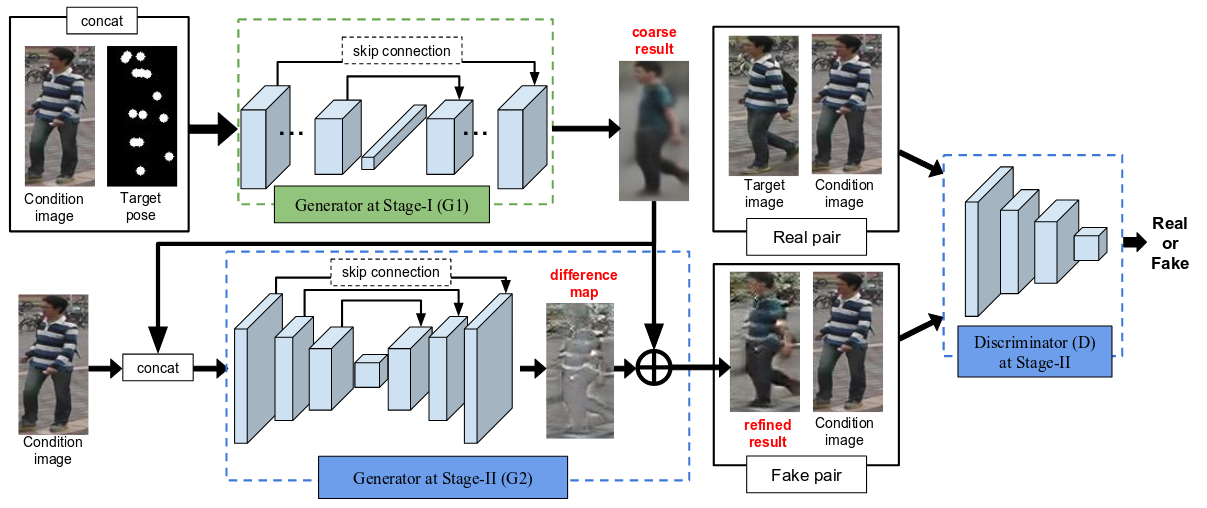
\includegraphics[width=8cm]{pose_guided.png}}
\caption{System architecture proposed by \cite{ref:pose_guided}.}
\label{fig:pose_guided}
\end{figure}

\subsection{Concepts from Complex Systems}
\label{subsec:complex_systems}
My interest in the field of computer animation is what sparked my desire to
tackling one of the hardest problems studied therein; that is, given any 3D scene
predict what will rendered to the screen. The problem does not sound too
difficult, since the types of data for the scene is finite; however if we
consider the infinite number of possible interactions within the scene itself,
the problem space grows exponentially.

In order to facilitate discussion on how the field of Complex Systems relates to
my project, I would first like to provide a definition of a ``complex system''
based what we studied in class:

\blockquote{
A complex system is a system made up of small components interacting with each
other to produce emmergence and to create global phenomena without a centeralized
controller. The system must also adapt to context and environment, meaning it is
impossible to predict the state it is in even if we were to know all laws
affecting the system and all initial starting conditions; the system is
nonlinear by nature of its complexity.
}

I believe my project abstractly encapsulates all the qualities of a complex system;
we are not concerned with the state of the animation software, but rather the
complexity of predicting the pixels that make up a rendered frame of an
animation. What is displayed by these pixels is completely dependent upon how
the objects in the scene interact with one another, however at times it is difficult
to find these interactions.
Anomalies such as these create the emmergent behaviour that makes 3D animation so rich
an artform.

What might we consider as the ``global phenomena'' for a 3D scene?
To answer this question, we must examine the various parts that make up a scene.
We are only concerned with components that impact the visual rendered by the
camera, and so components such as scripts, heirarchy data, etc. can be safely
excluded from consideration. Any physical objects, including meshes, particle
systems, lights, and cameras, contain valuable information pertinent to
what will be rendered; material attributes (e.g. opacity, reflectivity, or emission),
physical characteristics (e.g. size, shape, or behaviour), and animated movement can all
impact the rendered pixels for other objects in the scene. Essentially, what is rendered to the
screen is a combination of all of these characteristics for each object.
This behaviour increases the visual richness of what is rendered, however in the
same way also increases the complexity of defining how objects interact with
each other. After also considering the limitless possibilities for the objects
in a 3D scene,
it becomes clear that no iterative algorithm will ever be good enough
to provide a solution to this problem. Therefore this problem is
nonlinear and requires an abstract nonlinear approach in order to be solved.

\section{Architectural Overview}
\label{sec:architecture}
The architecture I outline here is based off of the research presented in
\cite{ref:pose_guided}. As I mentioned before, this architecture has several
components which I believe are important to my system. Below I outline the three
most important components which I plan to include in my architecture (see Figure
\ref{fig:block_diagram} for a block diagram of my architecture):

\begin{enumerate}
\item Generator I: uses a Convolutional Nueral Network (CNN) model to generate a
low resolution image containing global structures found in the
source data. This generator will likely be the most important component to
research, since I have not found a previously developed model to best suit the
generator's purposes. To accomplish my desired end result,
I believe I will need to combine the research of the LSTM
model from \cite{ref:frame_prediction} with the
generative CNN models from \cite{ref:pixelcnn_decoders}, \cite{ref:pixelcnn++},
and \cite{ref:multi_source}, and the research of semantic data from
\cite{ref:image_captioning} and \cite{ref:posecnn}. Because of the apparent
level of developmenet necessary for this compoenent, I have
outlined it in orange as shown in Figure \ref{fig:block_diagram}.
\item Generator II: uses a fully connected CNN with the output of the first generative network and a
condition image to generate a detailed output suitable as pixels of a rendered
frame. I believe this network will be easier to construct than the model for the
first generator, since it is likely I will be able to use roughly the same approach as
\cite{ref:pose_guided} did for their second generative network. One difference I
predict is the necessity for training data spanning multiple frames, which again
could touch on the LSTM model presented in \cite{ref:frame_prediction}.
\item Discriminator: trains a network to recognize a fake image from a real
image, thereby driving both generators to do a better job of creating their
respective outputs. This component is very well-researched by current standards,
and I should have little difficulty replicating the work of
\cite{ref:pose_guided} in order to create a working discriminator.
\end{enumerate}

\begin{figure}[htbp]
\centerline{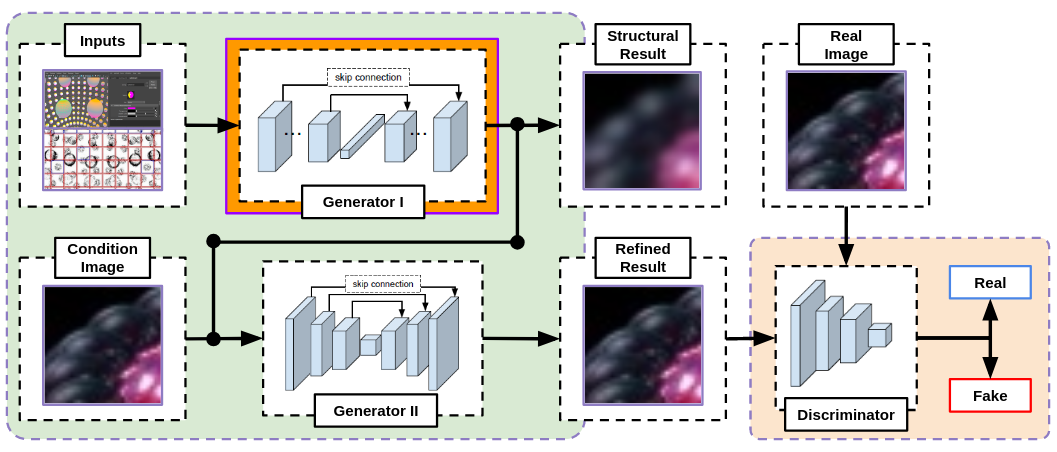
\includegraphics[width=8cm]{block_diagram.png}}
\caption{Block diagram for proposed architecture.}
\label{fig:block_diagram}
\end{figure}

\section{Project Considerations}
\label{sec:considerations}
For my project this term, I focused on creating the inputs of my target
architecture. In the following subsections, I ellaborate
on the reasoning for how these inputs are difined. This work is essential to my
proposed system, since the generator/discriminator model is useless if input
training data is not representative what what we'd like to be generated.

\subsection{A discussion on system inputs}
\label{subsec:inputs}
A major subarea of research for this project is how to generate the
information from a 3D scene that would be valuable to the proposed architecture
(see Figure \ref{fig:block_diagram}).
When first researching this topic, I posed the question of what
data should be sent to Generator I of the system.
In the research they present in \cite{ref:pose_guided},
Ma et. all uses a state of the art pose recognition program to
create image masks as extra input to their generative model.
The program assigns 18 ``keypoints'' for each pose,
which are then used as the pose representations for each iteration.
The pose data can be represented as a black and white image,
as shown in Figure \ref{fig:pose_guided}.
Disregarding the architectural changes to the generator, I predict I too will
have similar inputs; one or more frame image/scene data pairs for each iteration.

The pose data is not mapped one-to-one with my problem, however;
to solve the problem of reflective, transparent, and other dynamic surface attributes
I need the renderer to use all data in the scene.
If the camera is facing a mirror, for example,
then the entirety of the scene to be rendered is behind the camera.
Therefore, unlike with \cite{ref:pose_guided}
I found that using images as input would not work well for this problem,
unless the image abstractly captures the scene data relative to the camera and
the objects within the rendered view.

However, serializing every attribute of the scene for each frame would take too much time
and result in a bloated file size.
Using too little data could also produce poor results when training the
generator. Thus there are some requirements for this extra data, which I
outline below:

\begin{enumerate}
\item Data must be small in size but representative of the objects which it
describes. If any characteristics of the scene are left out of this
description, the trained algorithm may produce incorrect results in practice.
\item Data must also uniquely represent the objects in the scene and how they
interact with their environment.
If there is an abundance of similarities between objects, then
the algorithm might never learn the differences between the input frames.
\item There are no limitations nor expectations placed upon the animator;
even when comparing scenes which have similar characters, landscapes, and
animations, the generated data for each object should accurately represent
the properties of that object's relationship with the scene. If all the objects in the scene are the
same, then the focus would be on how they interact with each other in the scene
during animation.
\end{enumerate}

Given the above requirements for the input data,
I believe it is apparent not all pixels should be trained on, especially if they have
little to do with how the rendered scene is changing.
If pixels are paired with scene data for which they don't impact, the aspects of
the scene that are impacted will be recognized less accurately by the model.

In order to generate proper inputs,
a preparation phase is necessary for all frames of a given
animation. This process will involve selecting portions of each frame
to become system inputs.
I have defined these portions as ``frameblocks''.
Frameblocks represent a small ($\approx 3\%$) portion of a given frame,
and it is assumed
that a frameblock is representative of the changes between
two frames that are significant enough to
be included in the training set of inputs.
This concept of frameblocks also satisfies the
requirements enumerated in Section \ref{subsec:inputs}.

The selection of frameblocks depends upon how much the scene changes
between frames and in what ways it changes.
It is also pertinent that the inputs
take into account both scene data and rendered pixels;
as with complex particle systems, simply existing in the scene is all that is
needed to create great changes in the rendered output.
Therefore we cannot rely on scene data in our selection of frameblocks, rather
this selection must come from the changes in the frames themselves.
Scene data must then be linked to each selected frameblock, so that there is a
pairing between pixel and scene data.

%They are defined below (frames are indexed by $f_i$ for $i = 1,2,...,n$ where $n$ is the number
%of frames to train on):
%\begin{enumerate}
%\item The first frame, $f_1$, is automatically queried
%since it provides a baseline for changes shown in subsequent frames.
%\item The rest of the frames are processed as follows:
%\begin{enumerate}
%\item Frame $f_i$ 
%\end{enumerate}
%\item For each subsequent frame $f{i=2...n-1}$, the respective pixel values for
%frame $f_i$ and $f_{i - 1}$ are XOR'ed, and these results are summed together
%(perhaps the summation could be capped at 255, in order to save memory).
%\end{enumerate}
%This new composite image contains data on what has changed between frames,
%and it is to be evaluated by the Phase 1 Machine Learning algorithm to determine if the frame has enough changed values.
%But we should ask ourselves, is a Machine Learning algorithm necessary at this point?
%Surely we could just use the ratio of dark pixels to light pixels to make this decision.
%As stated before we are not only concerned with how much the frame changed overall but how it changed and where it changed.
%There is a problem with using frames that change too much, especially if the frames could be classified as separate scenes;
%each scene must be processed separately.
%Thus the decision of whether or not to use a given frame block for the current scene should be a trained decision,
%where the training data comes from similar analysis of movie frames where the scenes and changing areas are clearly defined.
%
%\subsection{Buffer Frameblocks}
%\label{subsec:buffer_frameblocks}
%Concerning frameblocks, an important question still remains:
%how do we capture changes not significant enough to trigger a frameblock as
%described in sections \ref{subsec:inputs} and \ref{subsec:frameblocks}?
%It is for this reason that I created the 
%
%Even if we captured all blocks that changed, how many of those changes would be similar?
%Depending on the frame rate and how many blocks changed,
%it could mean that most of the same blocks had similar changes which don't need to be retrained by the program.
%Given that a scene could have several seconds, if not minutes, of correlated data at a time,
%it is only natural to crop out important portions of the scene to use for training.
%Therefore there must also be a dynamic mechanism to select which frames classify as part of the current ?scene? and of those frames which to use as inputs to train on.

\subsection{Training The Algorithm}
\label{subsec:training_the_algorithm}
Now we know what we'd expect to be the inputs of the system, but what is an
appropriate amount of data to create good training results?
Usually, for a Deep Learning project, 10's of thousands of small images
are required to create a well-trained algorithm.
How many frames would I need to process in order to generate an appropriate
number of training data? I turn now to the industry standards for frame sizes
and frame rates.

My research of frame resolutions leads me to believe that production-quality
renders are no less than 1080 x 1920 (reffered to as 1k) pixels, while for movie
theatres or HD displays frames could be as large as 2k or 4k, meaning a max
resolution of 4096 x 3072 pixels. I will assume for this project frames are the
minimum 1k resolution.

Framerates of 60 frames per second (fps) or higher is quite common for high quality gaming applications,
however these would not apply to my project since game rendering must ocurr in
real-time.
Instead, I focus on the standard for animation frame rates, which was found to
range from 24 to 30 fps. I'd like to focus on 24 fps which is the minimum
standard I found.

Let's assume that 32 x 32 pixel frameblocks are sufficient for each image in the
training set.
Assuming the 1k resolution, there are then roughly 33x60 frameblocks available per frame,
or 1980 created blocks total.
Similarly, if we assume there is a rate of 24 fps and that every other frame is
rendered,
that leaves 23,760 possible frameblocks per second.
Now we can finally conjecture as to how many seconds of rendered data would be
worth using this approach.
Given that the number of frameblocks generated as described in Section
\ref{sec:implementation} could be much less than half of those available on
average, I assume that each frame has an average of 5\% of frameblocks passed
on to the training set. Thus, each second there are roughly 1,188 frameblocks
generated. So to reach at least 10,000 images or more, we would require around
10 seconds worth of animated data.
The animation I used this term contained 13 seconds of 1k resolution data and generated
a total of 14,330 frameblocks, which lines up nicely with my assumptions and
requirements for training.

%\subsection{Training Analysis}
%\label{subsec:training_analysis}
%However clustering is a problem better suited for data with multiple unique qualities,
%much like a problem for n-dimensional space.
%This data does not represent anything more than the amount of difference between two frame's pixels.
%The argument can be made that there may be waste in the frameblocks; take for example if a
%frame block edge straddles an area that just barely meets the criteria for processing while neither frame block will be processed.
%So a set configuration is ineffective for selecting frameblocks, since there may be missing frames in the selection.
%What about a sliding window? But then by how much should this window slide by? And what if there is too much overlap between frameblocks selected?
%Well if there is too much overlap, too many of the same frame will be selected and the algorithm can overtrain.
%If there is too little coverage, then frames will be missing.
%The solution? Perhaps a window that slides by half the width of a frame block, and half the height of a frame block.
%Should there be any extra rules to decide if a block indeed qualifies?
%For example, if two blocks are chosen because they have the exact same changes shown in both, should one of them be discarded?
%And should frameblocks be optimized to show changes in the center instead of on one side?
%Perhaps the frame should be dynamically chosen based upon threshold, shifted by 1 pixel each time until the frame has enough changes shown.
%A summation of all pixel values of the frame block could be applicable,
%and once a frame is found the offset could be set to half the frame block width
%(and height, when next changing rows).
%
%I also feel that the changes should not be a set value either; perhaps it should be a percentage of the total change overall.
%Take for example a slowly changing gradient from one color to another (changing over multiple frames).
%We would like to include this, since it is an important lerp to show in the generated frame,
%however the changes would be continuous over the entire frame. This is a big problem!
%How do we manage to only capture the frames we need for each configuration?
%Perhaps previous frameblocks should be captured and hashed, so that similar frameblocks are not captured.
%To do this I propose we take the first 5 bits of each color value for hashing (so that the last 8 possible values are ignored).
%Thus there are 15 bits to hash per pixel, and 32 x 32 pixels. I should research further what type of hash could be done.
%Some data loss is ok, since we want to disregard frameblocks that are too similar.
%Then maybe values should be super-sampled (averaged?) in smaller blocks to create a smaller 15 bits x 8 x 8 pixel image to compare against.
%However how much similarity is acceptable? There are probably too many ways to create the generated 8 x 8 pixel image based off of the given frames.
%Either way, it is clear that some method of hash could be used to avoid training on repeated blocks.
%
%In summary, the total process would be 1) find the frame block (by so far an unknown method), 2) check frame against previously found frames, 3) generate frame block and add to hash list. When the frame is completely processed, clear the list of hashed frameblocks.

\section{Term Project Implementation Details}
\label{sec:implementation}
This term I implemented an application to select all available frameblocks
showing changes in an input set of rendered frames. The only assumption on the
set of frames is that either dimension is divisible by the size of frame blocks,
or otherwise the edges of the frames contain no necessary training data. Below I
describe each step of the algorithm, and show intermediate outputs with
discussion on their significance.

\subsection{Frame processing}
\label{subsec:frame_processing}
The process for generating frameblocks takes in an input of 2 images and
outputs all frameblocks which meet the image processing requirements discussed
in Section \ref{subsec:inputs}.
Given the two frames shown in Figure \ref{fig:frame_processing},
the algorithm decides what portions of them contain enough changes to trigger
use in the training set as a frameblock.
Frame processing is iterative, and in order to obtain the changes between two
frames every frame will need to be processed along with its neighbors.
Luckily, the previous frame will have already been calculated in the previous
step, so we only need to compare each frame to the next frame for frameblock
selection.

As shown by the implemention in Appendix A, the frames are
read in as an array and processed.
Boundaries are also chosen, in case the images are different sizes.
In practice this wouldn't occur since the frames of an animation are always the
same dimensions.
Figure \ref{fig:frame_processing} shows an example of the two input frames,
as a reminder of how different they appear (compare this to what is later
described as the pair's shadow image, discussed in Section
\ref{subsec:shadow_image_creation}).
In theory these images should be separated by a single consecutive frame,
which usually means they will have very small differences.

\begin{figure}[htbp]
\centerline{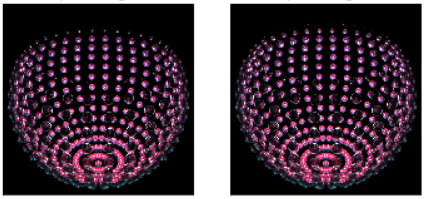
\includegraphics[width=8cm]{frame_processing.png}}
\caption{Frame processing comparision between 2 input frames.}
\label{fig:frame_processing}
\end{figure}

\subsection{Shadow image creation}
\label{subsec:shadow_image_creation}
At this stage of the algorithm the pixels of each image are processed.
A summation of pixel values is recorded for each pixel;
this sum adds the pixel's red, green, and blue (RGB) values together, and
caps the value at 255.
The goal is to record pixel $P(x,y)$,
which represents the difference between the two
pixels at the coordinates $(x,y)$ for each input image.
I call the image created out of the resulting pixels the "shadow image" for the two inputs.
For our purposes, let $p_i(x,y)$ represent the pixel at coordinate
$(x,y)$ for image $i$ and let $\oplus$ represent the XOR operation.
Thus for each cooresponding pixel of input image pair,
the following value is calculated:

$$P(x,y) = p_1(x,y) \oplus p_2(x,y)$$

The image made up of $P(x,y)$ for all $x,y$ ranging over the width and height of
the input images is output as the ``shadow image''.
Below is the calculated output image.
This image graphically shows the differences between frames,
where white represents no difference and black represents the maximal difference.
We are able to use this later to calculate frameblocks.

\begin{figure}[htbp]
\centerline{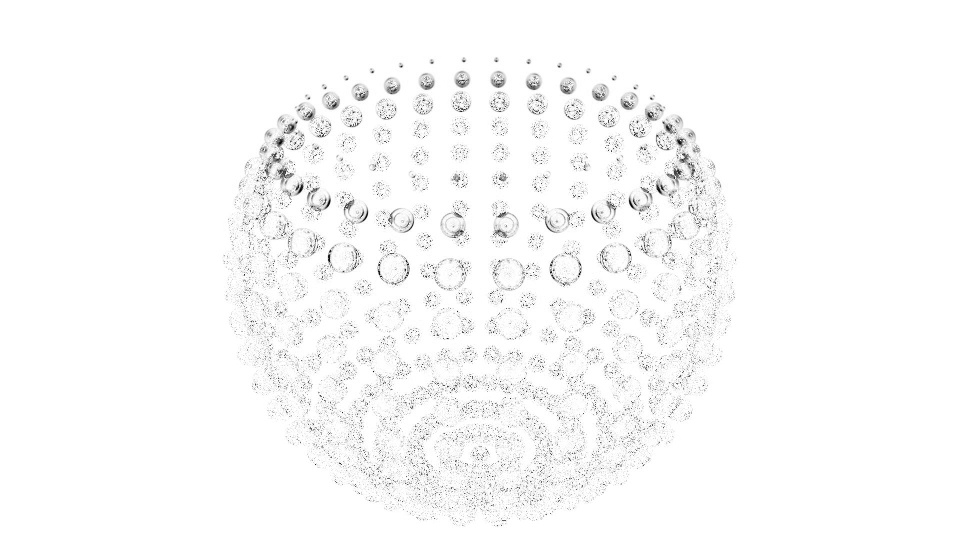
\includegraphics[width=8cm]{shadow_image.png}}
\caption{Shadow image produced between input frames shown in Figure
\ref{fig:frame_processing}.}
\label{fig:shadow_image}
\end{figure}

\subsection{Frameblock selection}
\label{subsec:frameblock_selection}
We select frameblocks using the above calculated image.
Frameblocks are selected based on the percentage of black pixels
(which in this case represents maximal difference).
To calculate the percentage of black pixels,
the total sum of pixel values in the shadow image is divided by how many black pixels are possible in the image.
Thus the value represents the probability of encountering a changed pixel between the two input images.
If the ratio calculated in this way is very low,
that means there are very few black pixels so we need to lower our standard for selecting frameblocks.
Similarly, if the ratio is close to 1,
that means there are many more black pixels and we should raise the standard for selecting frameblocks.
This value is directly tied to the input frames.

We need a sliding window to process frameblocks,
since we want to skip as many pixels of the same image as possible.
The overlap for each frameblock horizontally and vertically is given from the
block\_offset variable set in the beginning of the program.
A value of 1 means no overlap is possible,
a value of 2 gives 50\% possible overlap, and so on.

Each frameblock selected is saved to an image file.
A red rectangle is also overlaid on top of the original calculated image to represent where each frameblock was selected from.
Frameblocks which are found to not show enough changes to be included in this iteration are used to find differences spanning multiple frames (described later).

\begin{figure}[htbp]
\centerline{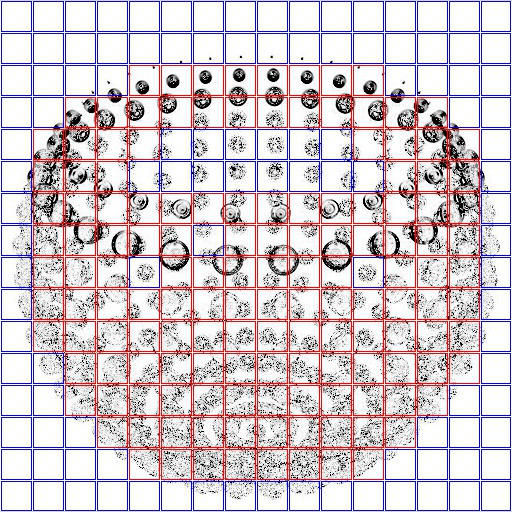
\includegraphics[width=8cm]{shadow_roi.png}}
\caption{Selected (red) and unselected (blue) frameblocks.}
\label{fig:shadow_roi}
\end{figure}

\subsection{Buffer frameblocks}
\label{subsec:buffer_frameblocks}
We stored the frameblocks that failed to pass the test this iteration in two formats:
an inverted shadow image file and a frame image file.
The shadow image file contains the calculated pixel\_sum for each pixel of the ROI of the original shadow image,
added together with any previous buffered frameblocks.
Thus each frameblock is not only a comparison between the current and next frames,
but instead a comparison of all the frames which didn't pass before.
It is clear to see from this that even if the change is gradual,
it will eventually be represented in the training data.
The ROI from the first input image is also saved so that this change can be accurately captured.
If the frameblock never changes enough over the entire course of frameblock generation,
it is not included in the dataset.
An example pair of inverted shadow and frame buffer images is shown below.

\begin{figure}[htbp]
\centerline{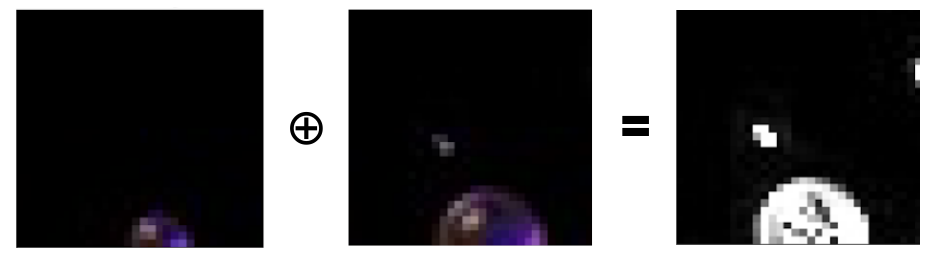
\includegraphics[width=8cm]{buffer_frameblock.png}}
\caption{Example of a buffer frameblock.}
\label{fig:buffer_frameblock}
\end{figure}

\subsection{Validation of experimental data}
\label{subsec:data_analysis}
The animation I used to test the application
contained 13 seconds of 1k resolution data and generated
a total of 14,330 frameblocks, which lines up nicely with my assumptions and
requirements for training. However how can we validate that the output frameblocks
accurately reflect the changes in the scene that should be captured?
I propose a comparison between these outputs and those generated from the same
scene with different properties.
As it so happens, the original scene is much more complex than we might have realized before.
Each sphere is transparent and very reflective,
so the changes to one sphere impact changes to all the spheres in the scene.
Since each the sphere's scaling and translation are changed throughout the
animation, the rendered sequence has lots of dynamic changes which should be
captured in frameblocks.
The process described above is repeated, but with
spheres that are completely opaque and diffuse.

\begin{figure}[htbp]
\centerline{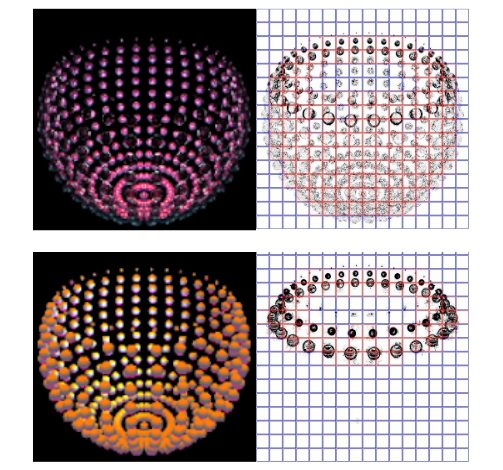
\includegraphics[width=8cm]{data_analysis.png}}
\caption{Comparison of complex (top) and simple (bottom) inputs.}
\label{fig:data_analysis}
\end{figure}

As can be seen in Figure \ref{fig:data_analysis}, the algorithm is able to filter
out more data and choose only frameblocks which change between the two frames.
This is exactly the desired outcome, since in both the complex and simple
scenes all changes are captured appropriately and no unnecessary frameblocks are
generated that could result in poor training data.

\subsection{A study on the discriminator model}
\label{subsec:discriminator}
Machine Learning stuff...

\subsection{Term project conclusions}
\label{subsec:term_conclusions}
The process discussed here is an effective means of choosing frameblocks
for training Generator I of the proposed framework in Figure \ref{fig:block_diagram}.
By carefully deciding which portions of the input frames to use,
it is guaranteed there will be minimal over-training of data and maximal changes shown in the dataset.
The implementation in Appendix A has proven to generate enough images for the
data training set.
The other input for the generator (i.e. the scene data) has not been decided yet.

\section{Future Work}
\label{sec:future_work}
The next step concerning input preprocessing will be to define how
scene data should be paired with the generated frameblocks.
Deciding what aspects of the scene to bundle with each
frameblock will require more research and experimentation;
it is possible that unique object masks may need to be rendered in order to
distinguish between objects inside of each frameblock.
Further work is also needed to complete the implementation of the discriminator;
I plan to apply what I learned from my study of the discriminator model, and
create a basic working generator/discriminator system which trains itself to
create realistic frameblocks. This simpler generator/discriminator system will
then be modified to accomodate the addition of scene data.

I have collected a small number of research papers which will help me solve this
problem and many others I will face.
\cite{ref:frame_prediction},
\cite{ref:spatiotemporal}, \cite{ref:posecnn}, and \cite{ref:pose_guided}
contain concepts that apply directly to my project.
Building upon the collection of cutting-edge research I uncover,
I intend to fully develop an appropriate system to address my problem statement.
After implemention and testing of the completed system is
accomplished, I plan to compile my research into a Master's Thesis with the
hopes of presenting my findings at conferences such as SIGGRAPH.

\section{Conclusion}
\label{sec:conclusion}
This term project presented many unforseen challenges. The foundation of this
idea was fostered
through the insights of CS 5790, Wearable Computing \& Complex Systems, via the
classroom discussions and reading assignments therein. I found these concepts to
be very applicable to many problems in the field
of Computer Graphics. At the start of the semester, I had hoped to simply provide a solid foundation
for beginning work on my thesis, however I did not believe I would come as far
as I have this semester alone. I succeeded in solving one of many problems I
will face for this project: the creation of image data for training a
basic generator/discriminator model. As discussed previously, I will build upon my
research and implementation to create a fully functioning frame prediction system.

Through the work I completed on this term project
I created an application to capture the changes
represented through an animated sequence in portions of rendered frames which I call
``frameblocks''. After discovering that my system lacked in representing gradual
changes, I increased the flexibility of it through the concept of ``buffer
frameblocks''. Once my implementation was complete,
I proved its worth by generating an adequate number of frameblocks for a
data set using a complex animation of 300 frames with 1080 x 1920 pixel
resolutions.
I was also able to validate my results
by comparing intermediate data to a simpler scene, and confirming that in all cases
the expected frameblocks were output by the application.
Finally I created a secondary application to separate the exported frameblocks
into a training, validation, and testing sets which will be used for the next
steps of my project. Although I did not complete an implementation of the
Machine Learning discriminator model, I feel my research into the topic provided
me with enough foundation to start working to meet this goal.

I learned so much throughout the course of this project, and I am very excited
to continue my work in the Fall of 2020. Over the summer I will continue to
collect conference papers and other research materials that might aid me in the
development of this project, and I look forward to overcoming the new challeges I will
undoubtedly face in the future. They will surely provide me with new and
exciting insights
into the fields of Computer Graphics and Complex Systems.

\begin{thebibliography}{13}
\bibitem{ref:bessel_functions} G. Eason, B. Noble, and I. N. Sneddon, ``On certain integrals of Lipschitz-Hankel type involving products of Bessel functions,'' Phil. Trans. Roy. Soc. London, vol. A247, pp. 529--551, April 1955.
\bibitem{ref:predictive_rendering} Alexander Wilkie, Andrea Weidlich, Marcus Magnor, and Alan Chalmers. 2009. ``Predictive Rendering.'' In ACM SIGGRAPH ASIA 2009 Courses (SIGGRAPH ASIA '09). ACM, New York, NY, USA, Article 12, 428 pages.
\bibitem{ref:frame_prediction} R. Mahjourian, M. Wicke and A. Angelova, ``Geometry-Based Next Frame Prediction From Monocular Video''. 2017 IEEE Intelligent Vehicles Symposium (IV), Los Angeles, CA, 2017, pp. 1700-1707.
\bibitem{ref:image_captioning} Oriol Vinyals, Alexander Toshev, Samy Bengio, and Dumitru Erhan. 2017. ``Show and Tell: Lessons Learned from the 2015 MSCOCO Image Captioning Challenge.'' IEEE Trans. Pattern Anal. Mach. Intell. 39, 4 (April 2017), 652-663.
\bibitem{ref:posecnn} Yu Xiang, Tanner Schmidt, Venkatraman Narayanan, Dieter Fox. ``PoseCNN: A Convolutional Neural Network for 6D Object Pose Estimation in Cluttered Scenes.'' CoRR abs/1711.00199 (2018): n. pag.
\bibitem{ref:pixelcnn_decoders} A\"{a}ron van den Oord, Nal Kalchbrenner, Oriol Vinyals, Lasse Espeholt, Alex Graves, and Koray Kavukcuoglu. 2016. ``Conditional Image Generation With PixelCNN Decoders.'' In Proceedings of the 30th International Conference on Neural Information Processing Systems (NIPS'16), Daniel D. Lee, Ulrike von Luxburg, Roman Garnett, Masashi Sugiyama, and Isabelle Guyon (Eds.). Curran Associates Inc., USA, 4797-4805.
\bibitem{ref:pixelcnn++} Time Salimans, Andrej Karpathy, Xi Chen, Diederik P. Kingma. 2017. ``PixelCNN++: Improving The PixelCNN with Discretized Logistic Mixture Likelihood and Other Modifications.'' ICLR Conference Paper (2017).
\bibitem{ref:multi_source} Eunvyung Park, Xufeng Han, Tamara L. Berg, Alexander C. Berg. ``Combining Multiple Sources of Knowledge In Deep CNN's For Action Recognition.'' 2016 IEEE Winter Conference on Applications of Computer Vision (WACV) (2016): 1-8.
\bibitem{ref:pose_guided} Liquian Ma, Xu Jia, Qianru Sun, Bernt Schiele, Tinne Tuytelaars, Luc Van Gool. ``Pose Guided Person Image Generation.'' NIPS (2017).
\bibitem{ref:multi_view} Bo Zhao, Xiao Wu, Zhi-Qi Cheng, Hao Liu, Zequn Jie, and Jiashi Feng. 2018. ``Multi-View Image Generation from a Single-View.'' In Proceedings of the 26th ACM international conference on Multimedia (MM '18). ACM, New York, NY, USA, 383-391.
\bibitem{ref:info_gan} Xi Chen, Yan Duan, Rein Houthooft, John Schulman, Ilya Sutskever, Pieter Abbeel. ``InfoGAN: Interpretable Representation Learning by Information Maximizing Generative Adversarial Nets.'' NIPS (2016).
\bibitem{ref:spatiotemporal} Christoph Schied, Anton Kaplanyan, Chris Wyman, Anjul Patney, Chakravarty R. Alla Chaitanya, John Burgess, Shiqiu Liu, Carsten Dachsbacher, Aaron Lefohn, and Marco Salvi. 2017. Spatiotemporal variance-guided filtering: real-time reconstruction for path-traced global illumination. In Proceedings of High Performance Graphics (HPG '17). ACM, New York, NY, USA, Article 2, 12 pages.
\bibitem{ref:monsters} Dean Takahashi, ``How Pixar made Monsters University, its
latest technological marvel''. April 24, 2013. Article.
\end{thebibliography}

\onecolumn

\begin{center}
\section*{Appendix A}
\label{app:a}
\end{center}

The following code is the contents of the
\mintinline{shell}{generate_frameblocks.py} project file, which is the
implementation file used to generate frameblocks.

\bigskip

\begin{minted}{python}
import os as os
import cv2 as cv2
import numpy as np

block_dim = 32
block_offset = 1

# Delete previously output frameblocks, and buffer shadows and buffer frames.
os.system('rm -rf %s' % './images/blocks/pairs/*')
os.system('rm -rf %s' % './images/blocks/buffer/shadows/*')
os.system('rm -rf %s' % './images/blocks/buffer/frames/*')

# Setup main loop to process all frames in an animation.
frames = os.listdir('./images/frames/')
frames.sort()

# Process each frame.
for frame_index in range(0, len(frames), 2):
  frame = frames[frame_index]

  # If the frame index is 0, store all frameblocks.
  if frame_index < 1:
    # Initialize seed variables.
    img_str_1 = './images/frames/' + frames[frame_index]

    # Choose smallest boundaries.
    img_1 = cv2.cvtColor(cv2.imread(img_str_1), cv2.COLOR_BGR2RGB)
    img_1 = cv2.resize(img_1, (0,0), fx=0.5, fy=0.5) 
    height, width = img_1.shape[:2]

    # Create sliding window.
    left = 0
    right = block_dim
    top = 0
    bottom = block_dim
    block_index = 1

    # Find the Region Of Interest (ROI).
    while bottom <= height:
      if bottom == height:
        bottom -= 1
      while right <= width:
        if right == width:
            right -= 1

        # ROI pixel processing
        print(str(block_index) + ". Frameblock: (" + str(left) + ", " +
          str(top) + "), (" + str(right) + ", " + str(bottom) + "))")
        
        # Setup storage.
        img_out_str = './images/blocks/pairs/block' + str(block_index)
                      + '/frame' + str(frame_index + 1)
        if not os.path.exists(img_out_str):
          os.mkdir('./images/blocks/pairs/block' + str(block_index))
          os.mkdir(img_out_str)

        # Store window contents as image.
        img_roi = img_1[top:bottom, left:right]
        cv2.imwrite(img_out_str + '/end.jpg', img_roi)

        # Increase frameblock index.
        block_index += 1
        
        # Shift horizontally.
        left += int(block_dim / block_offset)
        right += int(block_dim / block_offset)

      # Shift vertically.
      top += int(block_dim / block_offset)
      bottom += int(block_dim / block_offset)
      left = 0
      right = block_dim

  # Otherwise process as normal.
  else:
    # Initialize seed variables.
    img_str_1 = './images/frames/' + frames[frame_index - 2]
    img_str_2 = './images/frames/' + frames[frame_index]
    img_str_shd = './images/shadow/frame' + str(frame_index) + '.jpg'
    img_str_roi = './images/roi/frame' + str(frame_index) + '.jpg'

    img_1 = cv2.cvtColor(cv2.imread(img_str_1), cv2.COLOR_BGR2RGB)
    img_1 = cv2.resize(img_1, (0,0), fx=0.5, fy=0.5) 
    height_1, width_1 = img_1.shape[:2]

    img_2 = cv2.cvtColor(cv2.imread(img_str_2), cv2.COLOR_BGR2RGB)
    img_2 = cv2.resize(img_2, (0,0), fx=0.5, fy=0.5) 
    height_2, width_2 = img_2.shape[:2]

    # Choose smallest boundaries.
    height = height_1
    width = width_1
    if height_1 > height_2:
      height = height_2
    if width_1 > width_2:
      width = width_2

    img_out = np.ones((height, width, 3), np.uint8)

    # Calculate XOR image and pixel sum.
    print("Processing pixels of images, \'" + img_str_1 + "\' and \'"
           + img_str_2 + "\'")
    img_xor = cv2.bitwise_xor(img_1, img_2)
    pixel_sum = np.sum(img_xor)
    img_out = cv2.bitwise_not(cv2.cvtColor(img_xor, cv2.COLOR_BGR2GRAY))

    # Continue to next frame if no changes were found.
    if pixel_sum == 0:
      print("No changes found, continuing to next image.")
      continue

    # Write image.
    cv2.imwrite(img_str_shd, img_out)
    print("Wrote shadow image, \'" + img_str_shd + "\'")

    # Calculate the pixel_ratio.
    print("Total pixel sum: " + str(pixel_sum))
    pixel_ratio = pixel_sum * 1.0 / (255 * width * height)
    print("Pixel ratio: " + str(pixel_ratio))

    # Create a clone of input image and draw ROIs on top of it.
    img_roi_all = cv2.imread(img_str_shd)

    # Create sliding window.
    left = 0
    right = block_dim
    top = 0
    bottom = block_dim
    block_index = 1
    pixel_sum = 0
    cap = np.power(block_dim, 2) * 255 * pixel_ratio
    print("Cap found: " + str(cap))

    # Find the Region Of Interest (ROI).
    while bottom <= height:
      if bottom == height:
        bottom -= 1
      while right <= width:
        if right == width:
          right -= 1
        found_x = False
        dirty = False
        pixel_sum = 0
        img_buff_str = './images/blocks/buffer/shadows/block'
                       + str(block_index) + '.jpg'
        img_buff = cv2.imread(img_buff_str)
        if img_buff is None:
          img_buff = np.zeros((block_dim, block_dim, 3), np.uint8)
        
        # ROI pixel processing
        for y in range(top, bottom + 1):
          for x in range(left, right + 1):

            # Store buffer pixel and calculate pixel_sum.
            img_buff[y - top - 1, x - left - 1] += 255
                    - img_out[y, x]

            if img_buff[y - top - 1, x - left - 1][0] > 0:
              dirty = True
              if img_buff[y - top - 1, x - left - 1][0] > 255:
                  img_buff[y - top - 1, x - left - 1] = 255
            pixel_sum += img_buff[y - top - 1, x - left - 1][0]
            
            # Test if the cap was met.
            if pixel_sum >= cap:

              # Draw ROI on clone image.
              cv2.rectangle(img_roi_all, (left + 1, top + 1),
                           (right - 1, bottom - 1), (255, 0, 0), 1)
              cv2.putText(img_roi_all, str(block_index),
                         (left + 3, bottom - 3), cv2.FONT_HERSHEY_PLAIN,
                         0.75, (255, 0, 0), 1, 1)
              print(str(block_index) + ". Sum: " + str(pixel_sum)
                   + ", Frameblock: (" + str(left) + ", " + str(top)
                   + "), (" + str(right) + ", " + str(bottom) + "))")
              
              # Setup storage.
              img_out_str = './images/blocks/pairs/block' + str(block_index)
                            + '/frame' + str(frame_index + 1)
              if not os.path.exists(img_out_str):
                os.mkdir(img_out_str)

              # Store window contents as image.
              img_roi = img_2[top:bottom, left:right]
              cv2.imwrite(img_out_str + '/end.jpg', img_roi)
              
              # Exit both for loops.
              found_x = True
              break
          if found_x:
            break

        # If frameblock was used delete buffer shadow.
        if found_x:
          # If a buffered shadow image was used, delete it.
          if os.path.exists(img_buff_str):
            os.remove(img_buff_str)

          # If there is a buffered frame for the block use
          # it as the starting frame.
          img_buff_str = './images/blocks/buffer/frames/block'
                         + str(block_index) + '.jpg'
          if os.path.exists(img_buff_str):
            # Setup storage.
            img_out_str = './images/blocks/pairs/block' + str(block_index)
                          + '/frame' + str(frame_index + 1)
            if not os.path.exists(img_out_str):
                os.mkdir(img_out_str)

            # Move and rename file.
            os.rename(img_buff_str, img_out_str + '/start.jpg')

          # Otherwise export the ROI of the first image as the starting frame.
          else:
            # Setup storage.
            img_out_str = './images/blocks/pairs/block' + str(block_index)
                          + '/frame' + str(frame_index + 1)
            if not os.path.exists(img_out_str):
                os.mkdir(img_out_str)

            # Store window contents as image.
            img_roi = img_1[top:bottom, left:right]
            cv2.imwrite(img_out_str + '/start.jpg', img_roi)

        # Otherwise export the shadow and frame ROI to be used next time.
        else:
          # Draw Shadow ROI on clone image.
          cv2.rectangle(img_roi_all, (left + 1, top + 1), (right - 1, bottom - 1),
                       (0, 0, 255), 1)
          cv2.putText(img_roi_all, str(block_index), (left + 3, bottom - 3),
                     cv2.FONT_HERSHEY_PLAIN, 0.75, (0, 0, 255), 1, 1)

          # If the shadow image already exists, update it using a linear add.
          img_buff_str = './images/blocks/buffer/shadows/block'
                         + str(block_index) + '.jpg'
          if os.path.exists(img_buff_str):
            # Add the values of the current shadow image and previous shadow image.
            img_prev_buff = cv2.imread(img_buff_str)
            cv2.addWeighted(img_prev_buff, 1.0, img_buff, 1.0, 0.0, img_buff)

            # Store updated shadow image (don't update the old frame ROI).
            cv2.imwrite(img_buff_str, img_buff)
            print('Updated shadow image, \'block' + str(block_index) + '.jpg\'')

          # Else if a black pixel was found write a new shadow image.
          elif dirty:
            cv2.imwrite(img_buff_str, img_buff)
            print('Wrote new shadow image, \'block' + str(block_index) + '.jpg\'')

            # Store frame ROI image.
            img_buff_str = './images/blocks/buffer/frames/block'
                           + str(block_index) + '.jpg'
            img_roi = img_1[top:bottom, left:right]
            cv2.imwrite(img_buff_str, img_roi)

          # Otherwise notify that the block has been processed with no export.
          else:
            print(str(block_index) + ". No export")

        # Increase frameblock index.
        block_index += 1
        
        # Shift horizontally.
        left += int(block_dim / block_offset)
        right += int(block_dim / block_offset)

      # Shift vertically.
      top += int(block_dim / block_offset)
      bottom += int(block_dim / block_offset)
      left = 0
      right = block_dim

    # Write image.
    cv2.imwrite(img_str_roi, img_roi_all)
\end{minted}

\pagebreak

\begin{center}
\section*{Appendix B}
\label{app:b}
\end{center}

The following code is the contents of the
\mintinline{shell}{blur_frameblocks.py} project file, which is the
implementation file used to create training, validation, and test image sets for
training the discriminator discussed in Section \ref{subsec:derp}.

\bigskip

\begin{minted}{python}
import os as os
import cv2 as cv2
import numpy as np

home_dir = './images/'
blocks_dir = 'blocks/pairs/'
orig_dir = './training/validation/'
blur_dir = './training/blurred/'
keep_dir = './training/testset/'
blur_count = 1
keep_count = 1

# Delete previously output blurred frameblocks.
os.system('rm -rf %s' % orig_dir + '*')
os.system('rm -rf %s' % blur_dir + '*')
os.system('rm -rf %s' % keep_dir + '*')

# Setup main loop to process all frameblocks.
blocks = os.listdir(home_dir + blocks_dir)
blocks.sort()

# Process each block.
for block_index in range(0, len(blocks)):
  block = blocks[block_index]

  # Store all frames for that block.
  frames = os.listdir(home_dir + blocks_dir + block)
  frames.sort()

  # Process each frame.
  for frame_index in range(0, len(frames)):
    frame = frames[frame_index]
    img_in_str = home_dir + blocks_dir + block + '/' + frame + '/end.jpg'

    # Decide if image will be blurred or kept.
    flip = np.random.uniform(0, 1)
    if flip < 0.75:
      # Store end.jpg image to be blurred.
      img = cv2.cvtColor(cv2.imread(img_in_str), cv2.COLOR_BGR2RGB)

      # Skip image if entirely black.
      if np.sum(img) == 0:
          continue

      # Save original end.jpg image for validation.
      img_org_str = orig_dir + block + frame + '.jpg'
      cv2.imwrite(img_org_str, img)

      # Blur image.
      img = cv2.GaussianBlur(img, (7, 7), 0)
      
      # Output blurred image.
      img_out_str = blur_dir + block + frame + '.jpg'
      cv2.imwrite(img_out_str, img)
      print(str(blur_count) + ': 0 Blur ' + img_out_str)
      blur_count += 1

    else:
      # Skip image if entirely black.
      img = cv2.cvtColor(cv2.imread(img_in_str), cv2.COLOR_BGR2RGB)
      if np.sum(img) == 0:
          continue

      # Copy end.jpg image to testset.
      img_out_str = keep_dir + block + frame + '.jpg'
      cv2.imwrite(img_out_str, img)
      print(str(keep_count) + ': 1 Kept ' + img_out_str)
      keep_count += 1
\end{minted}
%==========================================================
\end{document}
%==========================================================
